\documentclass[conference]{IEEEtran}
\usepackage{cite}
\usepackage{array}
\usepackage{graphicx}
\usepackage{listings}	% Used to add code
\usepackage{float} %used to force figures in a position
\hyphenation{op-tical net-works semi-conduc-tor}

\begin{document}
\title{Building a Compilator on Java for a mini-C Programming Language}

\author{\IEEEauthorblockN{J. Agust\'{i}n Barrachina}
\IEEEauthorblockA{IEEE Student Member\\
\'{E}cole Polytechnique\\
Universit\'{e} Saclay-Paris}
\and
\IEEEauthorblockN{Phil\'{e}mon Poux}
\IEEEauthorblockA{\'{E}cole Polytechnique\\
	Universit\'{e} Saclay-Paris}}
\maketitle

\tableofcontents
\newpage

\begin{abstract}
In this project, a compilator was created to generate a x86-64 assembler code from a C fragment called mini-C.
This is a 100\% C-compatible fragment, in the sense that any Mini C program is also a C program. 
\end{abstract}

\IEEEpeerreviewmaketitle

\section{Introduction}
\textit{"Optimizing compilers are so difficult to get right that we dare say that no optimizing compiler is error-free! Thus, the most important objective in writing a compiler is that it is correct"}\cite{DRAGON_BOOK}

The reader is suppose to have some basic knowledge of C and for that reason almost no explanation regarding that language will be treated in this report. For further information about C language refer to \cite{LANGUAGE_C}.

Simply stated, a Compiler is a program that can read a code written in a specific programming language and translate it into an equivalent code of another language. A fairly good analogy can be made by a translator between two different languages like Spanish and French for example.

The objective of this project is to create a compiler for a fragment of C denominated \textit{Mini C}. Produce a reasonably effective code x86-64. In this project, a ".s" file will be created containing the translation between the C file to assembly. After the file is generated, the use of another compiler will be needed to produce the final output file that can be run by the computer. 

General knowledge of x86-64 assembly and the functioning of processors will also be required. The concept of the stack and registers like the callee saved and the caller saved must be clear for the reader.

\subsection{Mini C}
\subsubsection{What it does}
\textit{Mini C} is a fragment of the language C which contains integers and pointers to structures. \textit{Mini C} is 100\% compatible with C in the sense that every \textit{Mini C} program is also a C program. This will enable to use a C compiler such us \textbf{gcc} to use as reference. 

\textit{Mini C} can deal both with integers and structures. It can even support pointers inside structures to other structures or to the same structure in order to create lists for example. 

\subsubsection{What it doesn't}
%TODO: ADD STUFF NOT YET IMPLEMENTED. sizeof
\textit{Mini C} can deal both with integers and structures. But it doesn't work with any other types of variables such as floating point numbers or characters directly.

The function \textit{sizeof} is not yet implemented. The compiler will read it correctly and will know the program is correctly written but it will not know how to translate \textit{sizeof} resulting in an incomplete and broken assembly code.  

textit{Mini C} doesn't implement a for loop. Even though is almost the same as implementing a while loop. It was not believed to be relevant the implementation of it as an academic objective as the implementation of it will only require time but will not help in the better understanding of a compiler.

The "++" and "--" commands to increase or decrease a variables value were not implemented as well.

\subsubsection{Known bugs and work to be done} 
%TODO: add bugs

There was no real communication between the typer and the RTL (section \ref{sec:RTL}) generation code. For which reason, the toRLT function had to create in some cases some information already treated. This was not only working twice but also made the syntax class longer and more difficult to read. It is work for the future to create a better communication between both parts.

In the program, global structures were not yet implemented, although the code is prepared for it. In the section of code which it should be done, a throw error is prompt saying that the global structures are not yet implemented.

Although the compiler computes "$5 + 4$" directly as $9$, it will fail to do so when more complex integer operations are done like "$4 * 9 + (4 \&\& 0)$". It is to be done more optimization on this side. Jumps are also always done by the program itself and the compiler will not compute a "if(1)" as a direct jump to the section of code inside the if loop.

The division is not well implemented as it is done with whatever two registers desired, which will end up in an error compilation. Normally a division must be done between any register and \%rax, and to make the operation \(div r1 r2\) it is necessary to do:
\[ mov r2 \%rax\]
\[div r1 \%rax\]
\[mov \%rax r2\]
%TODO: format this thing.

\subsection{Structure of a Compiler}\label{sub_structure_of_a_compiler}

A compiler can be divided into two parts. The \textit{analysis} (front end) and the \textit{synthesis} (back end)

The \textit{analysis} brakes the source program into constituent pieces and imposes a grammatical structure of them in order to create a intermediate representation of the source program. During this part, syntactical formation and semantical unsound is checked. The analysis also collects information about the source program and stores it in a data structure called a \textit{symbol table} which will be used by the \textit{synthesis} part.

The \textit{synthesis} part makes use of the \textit{symbol table} and the intermediate representation constructed by the analysis part and creates the target program.

A more detailed diagram of the structure can be seen in figure \ref{fig_struct_of_compilator}. Where the last part (Code Generation) correspond to the \textit{synthesis} phase and the rest are all from the \textit{analysis} phase. The diagram is longer that the one displayed, having also a converser from the assembler to the machine language and from there to the executable code. But in this project, those stages are not treated.

\begin{figure}[H]
\centering
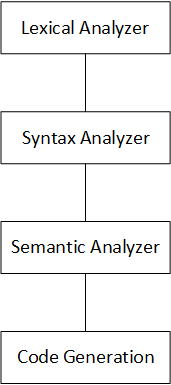
\includegraphics[width=3cm]{images/Diagram.png}
\caption{Structure of a Compiler}
\label{fig_struct_of_compilator}
\end{figure}

\section{Lexical Analyzer} \label{sec:lexical-Analizer}
A lexical analyzer (\textit{Lexer}) is the first front-end step in compilers, matching keywords, comments, operators, etc, and generating a token stream for parsers called \textit{lexemes} consisting of a \textit{token name} and the \textit{attribute value}. 
The \textit{token name} is an abstract symbol that will be used during syntax analysis, while the \textit{attribute value} is an entry in the \textit{symbol table} (discussed on \ref{sub_structure_of_a_compiler}) which will be used during the semantic analysis and the code generation.

The Lexer reads input from the programming language to compile (mini c in our case) and matches it against regular expressions and runs a corresponding action if such an expression is matched.

To make the Lexer are going to use:
\begin{itemize}
	\item Regular Expressions: To describe the lexemes
	\item Finite Automata: To recognize the expressions
\end{itemize}
\subsection{Regular Expressions}
The concept of regular expression arose in the 1950's when the American mathematician Stephen Cole Kleene formalized the description of a regular language.

A regular expression is a sequence of characters that define a search pattern. In other words, there are a conjunction of letters and digits that follow a certain rule.

Let us define \textit{letter} as any letter in the Latin alphabet and \textit{digit} any number [0-9]. Then we can define rules as follow: 
\begin{equation}
0 | [1-9] (<digit>* | [])\label{reg_expr_example}
\end{equation}

Last equation \ref{reg_expr_example} is a declaration of a decimal digit. The "$|$" is a logic or, it means, either the digit is 0 or it will be another thing. If it is not only 0, the number cannot start by 0 in C syntax, so it must start with a digit different from 0, which is range from 1 to 9 (encoded as [0-9]). Secondly, this digit can be followed by either nothing (represented by: []) or by any digit for as many digits are they must be. The format $<$rule$>$* means the repetition of a rule for as many times as necessary, or no repetition at all.

% We could add another example here, for example a comment line or sth.
\subsection{Finite Automata}
A \textit{finite automata} is basically a binary graph which just say "yes" or "no" by means of a \textit{recognizer} to each possible string.

There are two different classes of automatas:
\begin{enumerate}
	\item \textit{Nondeterministic Finite Automata} (NFA)
	\item \textit{Deterministic Finite Automata} (DFA)
\end{enumerate}
The first class (NFA) have no restrictions on the labels of their edges. A symbol can label several edges out of the same state. The DFA on the other hand have for each state and symbol exactly one edge with that symbol leaving that state. 
%translate to english...

\subsection{Implementation}

For the lexical analyzer, a flex library was used \cite{JFLEX}. A .flex file was created and then, by means of jflex, converted to the final java class.

Jflex lexers are based on a DFA automata. For more information about jflex library please refer to \cite{JFLEX_MANUAL}. 

The work of the lexer was only to read input from the file and create new symbols (\textit{lexemes}) containing the information as explained in \ref{sec:lexical-Analizer}.

\section{Syntax Analyzer} \label{sub_syntax_analyzer}

The syntax of a programming language describes the proper form of its programs.

The \textit{syntax analyzer} or \textit{parser} uses the first component of the \textit{lexemes}, the \textit{tokens}. The \textit{parser} creates some kind of tree representation that depicts the grammatical structure of the token stream called the \textit{syntax tree}. In this tree, each node represent an operation and the children of the node represent the arguments of that operation. 

\begin{figure}[H]
	\centering
	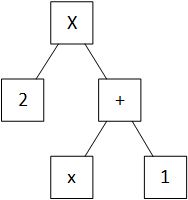
\includegraphics[width=3cm]{images/syntax_tree.png}
	\caption{Syntax Tree Example}
	\label{fig_syntax_tree_example}
\end{figure}

On figure \ref{fig_syntax_tree_example} an example of a tree representation can be seen. Many syntaxes can be the cause of that tree, for example, both \ref{(2*((x)+1))} and \ref{2*(x+1)} can be used to generate such tree.

\begin{equation}
2*(x+1)
\label{2*(x+1)}
\end{equation}

\begin{equation}
(2*((x)+1))
\label{(2*((x)+1))}
\end{equation}

\subsection{Implementation}

The Syntax Analyzer was done using CUP, a parser generator for java \cite{CUP}.

In that file, precedence where applied to each operator using the following table:
\begin{table}[H]
	\begin{center}
	\begin{tabular}{||c c||}
		\hline
		Operator & Associativity  \\ [0.5ex] 
		\hline\hline
		= & right \\ 
		\hline
		$|$$|$ & left  \\
		\hline
		\&\& & left  \\
		\hline
		== != & left  \\
		\hline
		$<$ $<$= $>$ $>$= & left \\ [1ex] 
		\hline
		+ - & left \\
		\hline
		* / & left \\
		\hline
		! -(negative) & right \\
		\hline
		-$>$ & left \\
		\hline
	\end{tabular}
	\end{center}
	\caption{Precedence} \label{tab_precedence}
\end{table}

The higher the operator is in the table, the last will it be applied. For example, the operator "=" will be applied after all the other operators have been applied. There is a very simple way to apply this table in the .cup file by simply writing the following command: precedence <associativity> <token name>. Where associativity is either left or right and the token name is the token from the \textit{lexem} created by the Lexer.

After the precedence, the following grammar was implemented (table \ref{tab_grammar}). The details on how to implement it where omitted. In order to see how to implement the following grammar in cup please refer to the user manual \cite{CUP_MANUAL}.

\begin{table}[H]
	\begin{center}
		\begin{tabular}{ | m{1.5cm} | m{6.5cm}| } 
			\hline
			$<$ file $>$ & $<$ decl $>$* EOF \\ 
			\hline
			$<$ decl $>$ & $<$ var $>$ $|$ $<$ type $>$ $|$ $<$ funct $>$ \\ 
			\hline
			$<$ var $>$ & int $<$ ident $>^{+},$ ; \newline 
						struct $<$ ident $>$ ( *$<$ ident $>^{+},$ ) ; \\ 
			\hline
			$<$ type $>$ & struct $<$ ident $>$ { $<$ var $>$* } ; \\
			\hline
			$<$ funct $>$ & int $<$ ident $>$ ( $<$ param $>^{*},$ ) $<$ bloc $>$ \newline 
							struct $<$ ident $>$ * $<$ ident $>$ ($<$ param $>^{*},$) $<$ bloc $>$ \\
			\hline
			$<$ param $>$ & int $<$ ident $>$ $|$ struct $<$ ident $>$ * $<$ ident $>$ \\
			\hline
			$<$ expr $>$ & 	$<$ integer $>$ \newline 
							$<$ ident $>$ \newline
							$<$ expr $>$ -$>$ $<$ ident $>$ \newline
							$<$ ident $>$ ( $<$ expr $>^{*},$ ) \newline 
							! $<$ expr $>$ $|$ -$<$ expr $>$ \newline
							$<$ expr $>$ $<$ op $>$ $<$ expr $>$ \newline
							sizeof ( struct $<$ ident $>$ ) \newline
							( $<$ expr $>$ )	\\
			\hline
			$<$ op $>$ & = $|$ == $|$ != $|$ + $|$ - $|$ * $|$ / $|$ \&\& $|$ $<$ $|$ $<$= $|$ $>$ $|$ $>$= $|$ $|$$|$ \\ 
			\hline
			$<$ instr $>$ & ; \newline
							$<$ expr $>$; \newline
							if ( $<$ expr $>$ ) $<$ instr $>$\newline
							if ( $<$ expr $>$ ) $<$ instr $>$ else $<$ instr $>$ \newline
							while ( $<$ expr $>$ ) $<$ instr $>$ \newline
							$<$ bloc $>$ \newline
							return $<$ expr $>$; \\				
			\hline
			$<$ instr $>$ & { $<$ var $>*$ $<$ instr $>*$  } \\
			\hline
		\end{tabular}
	\end{center}
	\caption{Grammar} \label{tab_grammar}
\end{table}

Where '$|$' is either one or the other is found. The '*' is as many as necessary (including none at all), while on the other hand, '+' means as many as necessary but at least one. If under any of those symbols there is a comma (',') it means there are comma indented.

As an example on how to read the table, wwe can see that within a file, one will find a list of declarations. These declarations can be either a variable  (global variables) or a structure declaration or functions. The declarations of functions have it's own parameters (or none) and a bloc in which it will be the code.
The bloc is composed by the declarations of the variables followed by instructions. The instructions are loops such as if or while or simply expressions. Expressions can be all type of C \& C ++ expressions such as integers, pointers, negation, call to functions, etc.   

\section{Semantic Analyzer} \label{sec:semantic-analyzer}
\textit{"Well typed programs do not go wrong"}

The semantics of a programming language defines what each program does when executing.

A \textit{Semantic Analyzer} uses the \textit{syntax tree} and the information in the \textit{symbol table} to check the source program for semantic consistency with the language definition. 

An important part of the \textit{semantic analysis} is the \textit{type checking} where it gathers type information and checks that each operator has matching operands.
An example of the type checking will be to make sure the index which whom an array is accessed is an integer and not any other incompatible type.
In a equation like \(8.0 + 4\), the type checking will make sure to convert the integer "4" into a floating point before making the operation. 

The \textit{type checking} will make sure that the variables of a equation like \(e1 + e2\) are from the same type and reject the incoherent programs. 
There are some languages that use \textbf{dynamic types}, which means they check they check the type of the variables dynamically. Such languages are for example PHP, Python or Lisp. On the other hand, there are also \textbf{static types} languages which is the compiler the one in charge on checking the types. For example OCaml, Java and C (which will be our case).

\subsection{Implementation}
The bigger and more critic class of the entire program was created in \textit{Syntax.java} class. An object of the class \textit{File}, created by the parser (which uses the lexer) implements a method called \textit{Typer} which takes care of what was explained in this section (\ref{sec:semantic-analyzer}).

%TODO: something to add?

\section{Code Generation}
In this section we will actually generate the assembly code itself. It takes as input an intermediate representation of the source program and maps it into the target language. 
It is too difficult to be able to do this part in only one step. So it will actually be divided into 3 stages:
\begin{enumerate}
	\item \textit{Register Transfer Language} (RTL)
	\item \textit{Explicit Register Transfer Language} (ERTL)
	\item \textit{Location Transfer Language} (LTL)
\end{enumerate}
Each stage will be explained in their corresponding sub section.

\subsection{Register Transfer Language (RTL)} \label{sec:RTL}
For this stage we will use the \textit{syntax tree} created on \ref{sub_syntax_analyzer} in order to create what will be called as \textit{RTL tree}. We suppose that the local and global variables are already differenced and that the type of each variable recognized as it has been done in the last section.

The main objective (more precisely the first part) of the RTL is to create a set of instructions x86-64 from the operations of C.

The second phase is to create a a \textit{Register Transfer Language}. Here a \textit{Control Float Graph} (CFG) is created that will facilitate the ulterior phases and that will eliminate the distinction between statements and expressions. This RTL will create the so called pseudo registers, which are an infinite number of intermediate registers to realize operations. This registers will be converted into actual x86-64 registers in the future.

\subsubsection{Implementation}
Each file contains a list of declarations of functions (as can be seen on table \ref{tab_grammar}) that contains a bloc statement. Each function, contains a list of parameters and the list of declarations of variables.
A RTL graph is created for each function in a recursive way. As seen in table \ref{tab_grammar}, a function has a list of statements that will be converted into one or more assembler commands. For each command, a label will be created and saved into the RTL graph, the RTL graph will contain each assembly operation with a label of reference to it. 

Each \textit{statement} and \textit{expression} class (declared in the syntax.java file) will have a "toRTL" method that will save it's label into the graph. The function "toRTL" will have as arguments:
\begin{itemize}
	\item \textbf{Register} Register to be used.
	\item \textbf{Exit Label} The label to which the program will go after making the current instruction.
	\item \textbf{The RTL graph which will be added} In case it is necessary to add two instructions or more which is almost always the case.
\end{itemize}
Later on, there were added some more information to the function to be able to work with variables and structures.
\begin{itemize}
	\item \textbf{Variables} Is a Map that links a string with it's register. This is used to know in which pseudo-register each variable is stored in order access it. If the variable is not there, it is supposed to be global. The Typer section will make sure the global really exists.
	\item \textbf{Struct Defintion} Is a Map between a string (the structure name) and a list of strings which are all the variables inside the structure. This is used for knowing what number to add as an offset when doing something like $p->a$
	\item \textbf{Struct Declaration} This is a Map between all structure pointers and the structure they are actually pointing. To actually compute $p->a$ first it will be necessary to use the structure declaration to know which structure is it pointing and then use the structure definition to know the offset. Because of the typer, this Maps will always contain what is is looking for, but an extra level of security was add to display an error if some variable is not in the Map.
\end{itemize}
The RTL function will return it's own label to be given to the next toRTL call in order to line up every statement and expression.

To make \textbf{condition branches}, another function will be created called "toRTLc" which will receive two label, one to be done if the expression is true, and another in order to be done in the other case. The structure will be represented as toRTLc(e, s1Label, s2Label) where 'e' will be the expression with a true or false value. s1Label will be the label to go if 'e' is true and s2Label in the other case.

In order to realize the \&\& expression, for example with the case:
"if e1 \&\& e2 do s1 else s2"
The following conversion will be done:
\[toRTLc(e1 \&\& e2, s1Label, s2Label) -> \]
\[toRTLc(e1, toRTLc(e2, s1Label, s2Label), s2Label)\]

Using a similar logic, the expression:
"if e1 $|$$|$ e2 do s1 else s2"
will be converted:
\[toRTLc(e1 || e2, s1Label, s2Label) -> \]
\[toRTLc(e1, s1Label, toRTLc(e2, s1Label, s2Label))\]

In order to make the \textbf{negative sign}, for example \(-2\), the compiler actually does the operation \(0 - 2\).

In order to make the \textbf{not operation}, for example !a. The compiler does an if statement such as:
"if a then 0 else 1".
In which case, making something like !!41 will return 1 as a result. Which is what actually happens in C code.

Some simplifications were done when doing binary operations. The compiler will compute the line:
\[ x = 4 + 5\]
as
\[x = 9\]

%TODO: put an example done by RTL it will be interesting

\subsection{Explicit Transfer Language (ERTL)}

The \textit{Explicit Register Transfer Language} is in charge of the function call conventions. Here, the first parameters are sent to a function are stored in the registers which convention dictates will be used (\%rdi, \%rsi, \%rdx, \%rcx, \%r8, \%r9) and the rest of the parameters will be stocked at in the stack. Also, it will return the result of the function in the register \%rax. It will also make sure the registers known as \textit{callee saved} are correctly saved by the function before returning to the previous function.

During this stage, some pseudo-registers will be converted to real registers.  

\subsubsection{Implementation}

Inside a class ERTL was created. The class implements a method called "createERTL" that receives an RTL class and creates an ERTL class from it.
Basically, the graph is maintained untouched except for the call to a function. There is also some extra code added to the beginning and the end of the function bloc.

A RTL function like this:

\begin{lstlisting}
#10 main[]
entry  : L15
exit   : L11
locals : [#8]
	L15: mov $42 #11 --> L14
	L14: #10 <- call fact[#11] --> L13
	L13: Mmov #10 #8 --> L12
	L12: Mmov #8 #9 --> L11
\end{lstlisting}

will now be extended to:

\begin{lstlisting}
main(0)
entry  : L32
locals : [#8]
	L32: alloc_frame --> L31 
	L31: Mmov %r12 #18 --> L30 
	L30: Mmov %rbx #17 --> L15
	L15: mov $42 #11 --> L14
	L14: Mmov #11 %rdi --> L29
	L29: call fact(1) --> L28 
	L28: Mmov %rax #10 --> L13 
	L13: Mmov #10 #8 --> L12 
	L12: Mmov #8 #9 --> L27 
	L27: Mmov #9 %rax --> L11 
	L11: Mmov #18 %r12 --> L35 
	L35: Mmov #17 %rbx --> L34
	L34: delete_frame --> L33 
	L33: return
\end{lstlisting}


\subsection{Location Transfer Language (LTL)}
\section{Conclusion}

% use section* for acknowledgment
\section*{Acknowledgment}

% Bibliography
\newpage
\IEEEtriggeratref{8}
\bibliographystyle{IEEEtran}
\bibliography{ref}

\end{document}


